\section{\textsc{IntraCFG}: Intraprocedural Framework for Source-Level Control-Flow Analysis}
The techniques of CFGs construction has seen significant advancements
in recent years, with various frameworks being proposed to aid in the construction 
of precise intraprocedural CFGs~\cite{smits2020flowspec,10.1016/j.scico.2012.02.002}.
We contributed to the state-of-the-art introducing \textsc{IntraCFG}, a declarative, RAG-based,
and language-independent framework for constructing precise intraprocedural CFGs.

Unlike most other frameworks, which build CFGs on an Intermediate Representation (IR) level,
such as bytecode, \textsc{IntraCFG}'s approach is unique in that it superimposes the CFGs 
on the Abstract Syntax Tree (AST). This allows for a more accurate client analysis,
as the CFGs are constructed directly on the source code level, rather than an
intermediate representation. Additionally, this approach also enables the construction 
of \textsc{AST-Unrestricted} CFGs, which are CFGs whose shape is not restricted to the AST structure.
\subsection{Overall Architecture}
The overall architecture of our proposed framework, \textsc{IntraCFG}, and its
ecosystem\todo{Not sure about the word ecosystem} is shown in Figure~\ref{fig:intraCFG}. 
The framework provides the skeleton and default behaviour for construction of CFGs,
which can be instantiated for specific languages\footnote{\textbf{\texttt{IntraX}} in the diagram.}, e.g., Java or Teal. 
\begin{figure}[H]
    \centering
    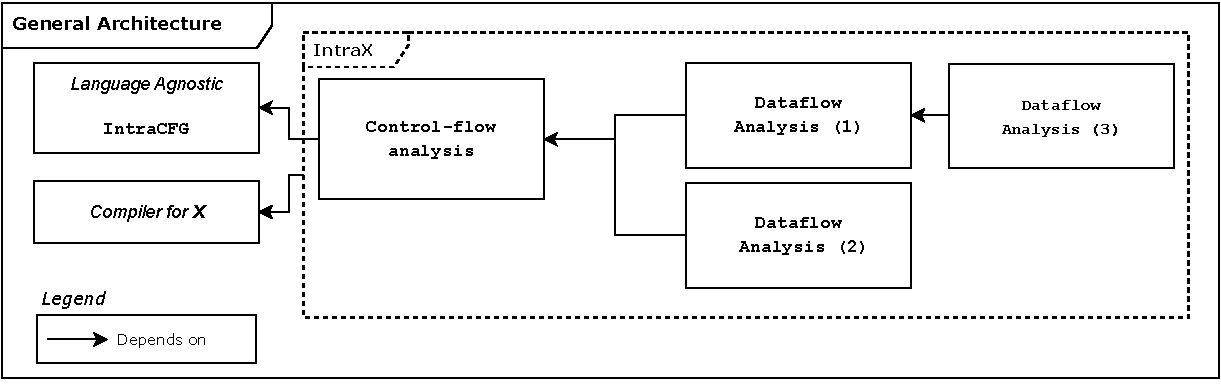
\includegraphics[scale=0.7]{kappa/img/architecture.pdf}
    \caption{\label{fig:intraCFG} Overall architecture of \textsc{IntraCFG} and its ecosystem.}
\end{figure}

The framework consists of several key components, including interfaces
(e.g., CFGRoot, CFGSupport, and CFGNode), attribute equations that define the
default behavior, and user APIs. The interfaces provide the structure for the
CFG and the attribute equations define the default behavior for the CFG
construction. Language specific AST nodes implement the different interfaces 
according to the level of precision desired for the CFG.
The APIs expose the CFG to the client analysis, and they are used to query the CFG
for information, such as the entry and exit nodes, or to traverse the CFG.
The language-independent nature of \textsc{IntraCFG} allows for easy integration 
with various programming languages and enables the construction of precise CFGs 
for those languages. The use of attribute equations and interfaces also allows 
for a high degree of flexibility in the CFG construction process, 
enabling the customization of the CFG to fit the specific needs of the 
analysis being performed.

Additionally, language-specific dataflow analysis, such as \texttt{NullPointerException} or
\texttt{IndexOutOfBound} detection, can be built on top of the framework.





\subsection{\textsc{IntraCFG} for Java}
To demonstrate \textsc{IntraCFG} applicability in a specific programming language, we developed
\textsc{IntraJ}, an instance of the framework for the Java programming language.
We built \textsc{IntraJ} as an extension of the ExtendJ extensible Java compiler~\cite{DBLP:conf/oopsla/EkmanH07}.
The complete architecture of \textsc{IntraJ} is shown in Figure~\ref{fig:intraJ}.
\begin{figure}[H]
    \centering
    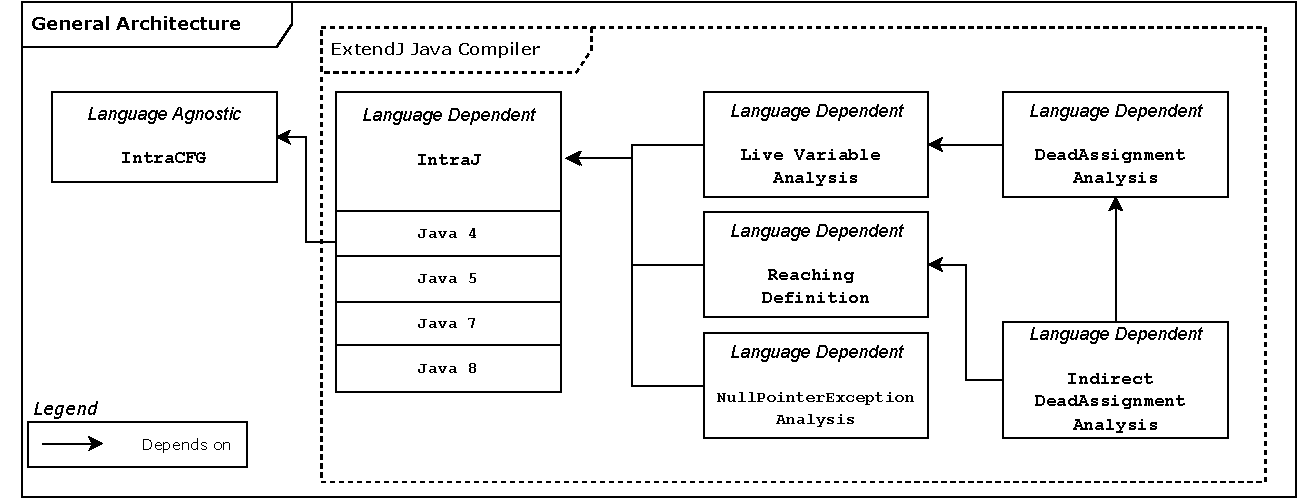
\includegraphics[scale=0.5]{kappa/img/architecturejava.pdf}
    \caption{\label{fig:intraJ} Overall architecture of \textsc{IntraCFG} instansiated for the Java language.}
\end{figure}

%Discussing modularity
We designed \textsc{IntraJ}, following a  modular approach, and we separately 
instansiated the framework for different versions of Java such as Java 4, 
Java 5, Java 7 and Java 8. Each version of Java is implemented as a separate
aspect of the compiler. This approach allows us and the users of \textsc{IntraJ}
to easily extend the framework to support new versions of Java.

% Discussing precision
The degree of precision in creating CFGs using \textsc{IntraCFG} can differ in order
to meet the requirements of a given application.
This flexibility allows us to optimize the efficiency of the analysis by selectively 
excluding certain nodes from the CFG, such as \texttt{WhileStmt}, which do not
provide any information relevant to the analyses. This leads in the reduction of
unnecessary complexity and with an overall improvement in the analysis's performance.
On the other hand, we can increase the precision of the CFGs by including more nodes
synthethizing new nodes and new subtrees. 
For instance, we designed \textsc{IntraJ} to compute an exception-sensitive 
control-flow analysis, i.e., new AST subtrees are synthesized for each exceptional path. 
The resulting CFGs are more precise, but they are also more complex, resulting 
in a higher memory consumption and a longer analysis time.
\begin{figure}[H]
    \centering
    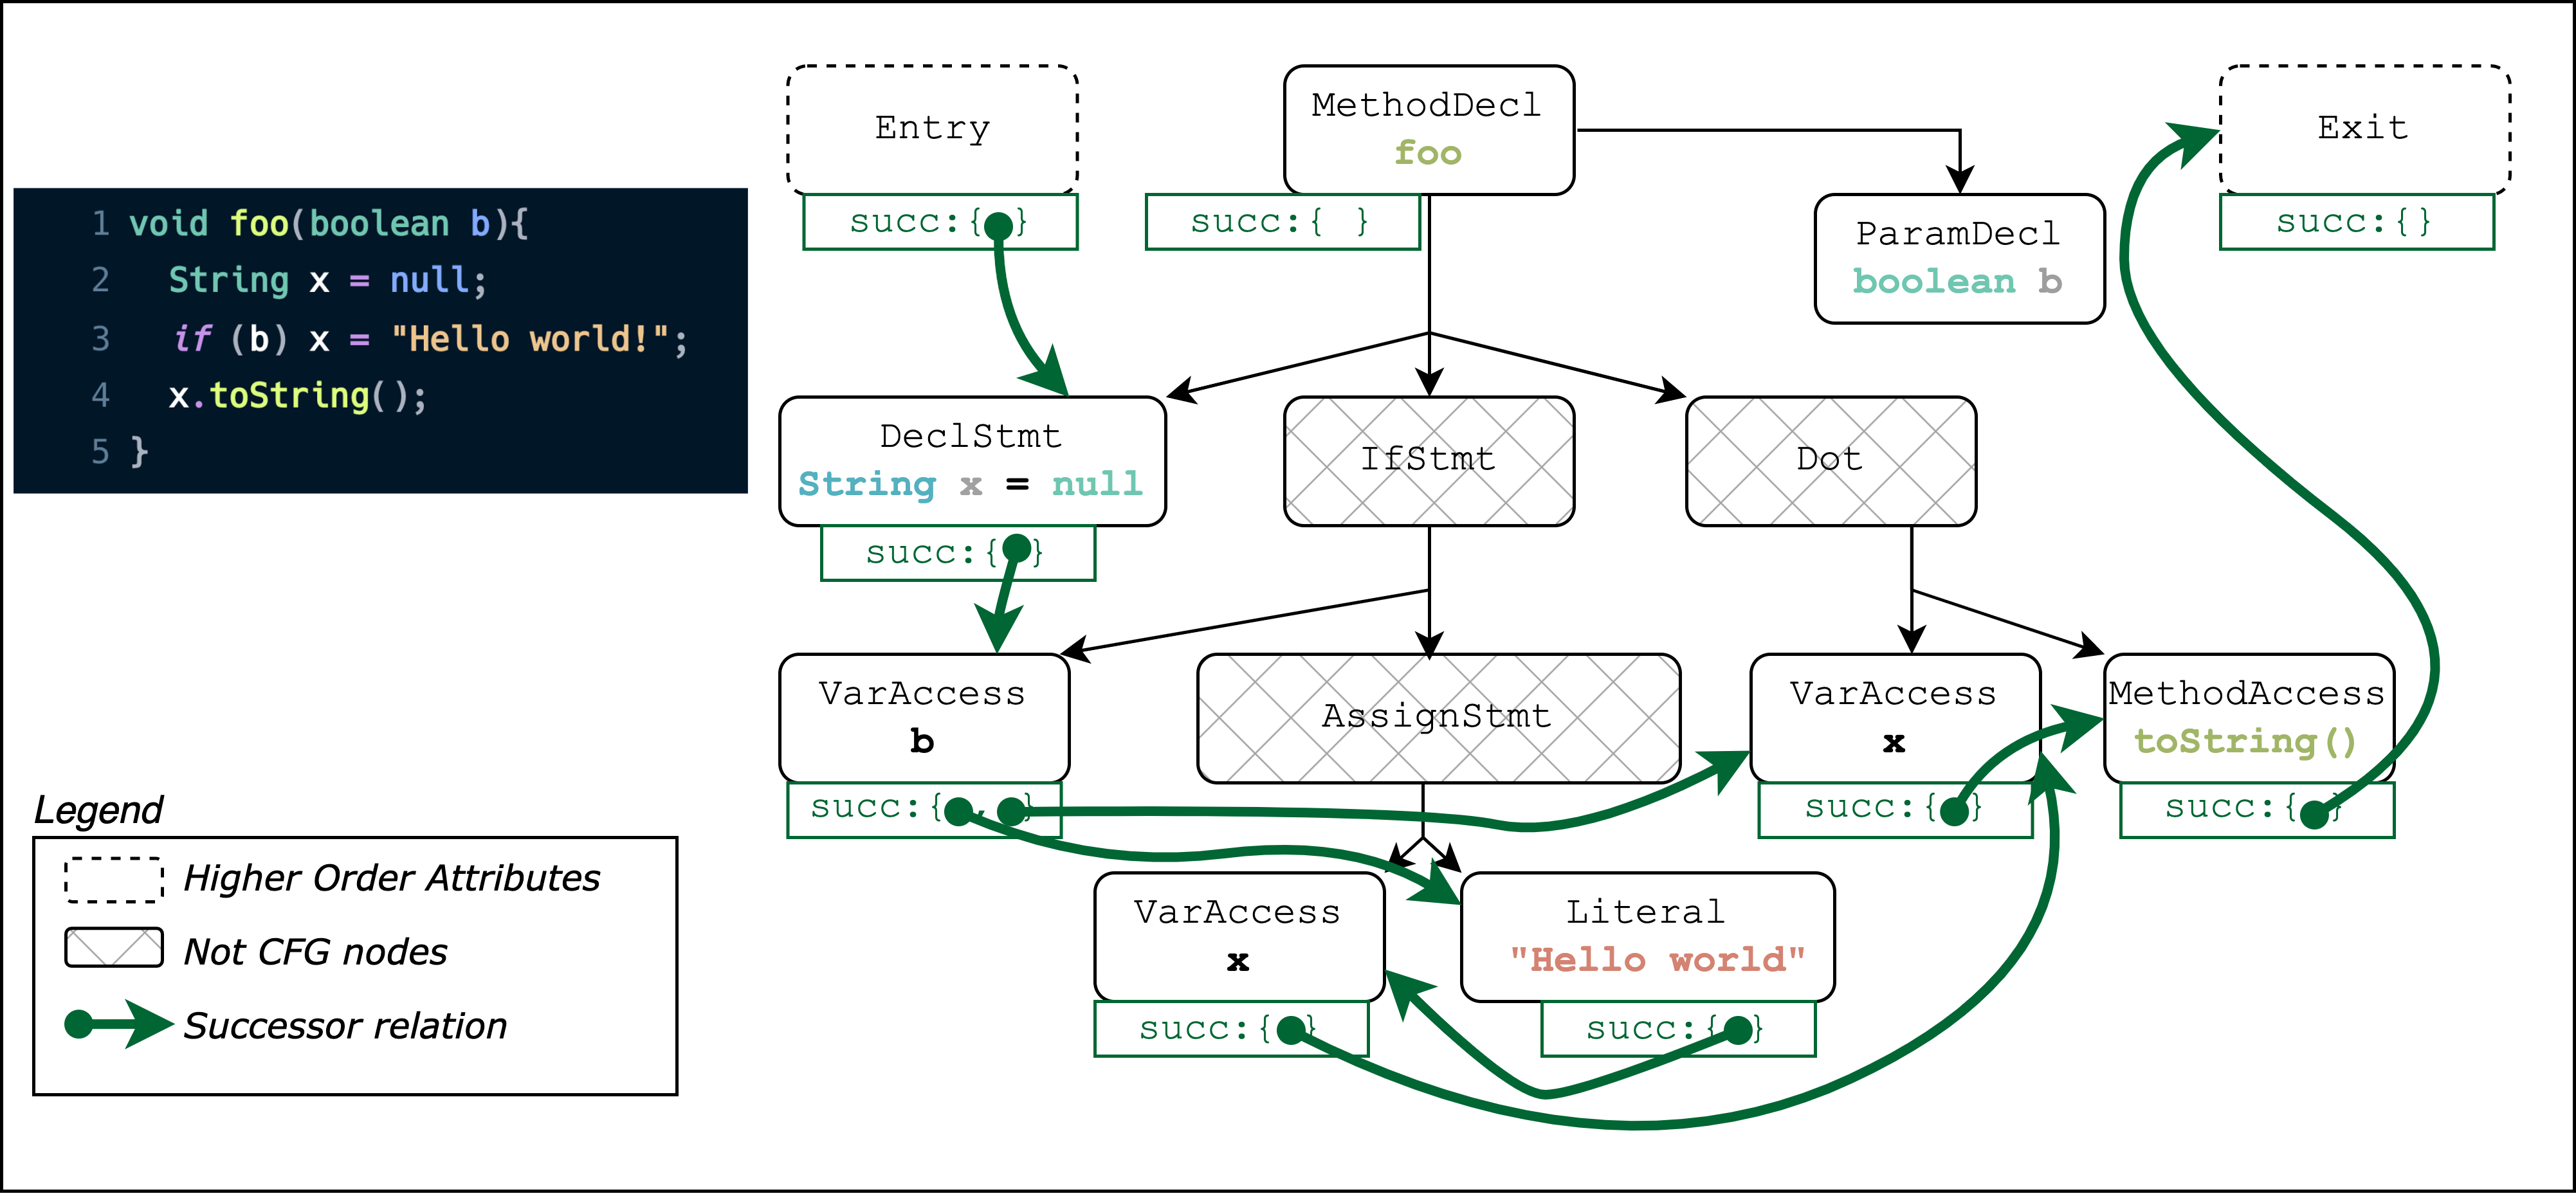
\includegraphics[scale=0.08]{kappa/img/exampleAST.png}
    \caption{\label{fig:CFG} CFG of the \texttt{foo} Java method.}
\end{figure}
The example in Figure~\ref{fig:CFG} is a visual representation of the AST and CFG of the 
\texttt{foo} Java method. The figure illustrates the ability of the framework to tailor the CFG
to the specific requirements of the analysis and eliminate unnecessary complexity for improved performance.
In this example, the \texttt{IfStmt} and \texttt{WhileStmt} and \texttt{AssignStmt} nodes are not included in the CFG,
resulting in a more concise but precise representation of the control flow of the program.


In \textsc{IntraJ}, we implemented five different dataflow analyses. The analyses 
relie on the result of the control-flow analysis. To the analysis are exposed 
the entry and exit nodes of the CFG, as well as the successor and predecessor
nodes of each node. 
Each analysis is implemented as a separate aspect of the compiler. Nevertheless,
the result of some analyses is used as input for other analyses. For instance,
the result of \emph{Live Variable Analysis} is used as input for the \emph{Dead Assignment Analysis}.
Similarly, the result of Dead Assignment Analysis is used to detect implicit dead assignments, i.e.,
assignments that are not dead but their use always flow to a dead assignment.

The analyses are implemented as instances of the Monotone Frameworks.
Each analysis defines its abstract domain, transfer function and \emph{in} and 
\emph{out}\footnote{Sometimes can be named \emph{gen} and \emph{kill}.} attributes.
The language dependency of the dataflow analysis arises from the fact that the
transfer function, which defines the relationship between the \emph{in} and \emph{out},
is modeled as an attribute. This transfer function attribute is 
define for each AST node in the CFG in order to capture the semantic of passing 
through that node.


















\subsection{\textsc{IntraCFG} for TEAL}
\begin{figure}[H]
    \centering
    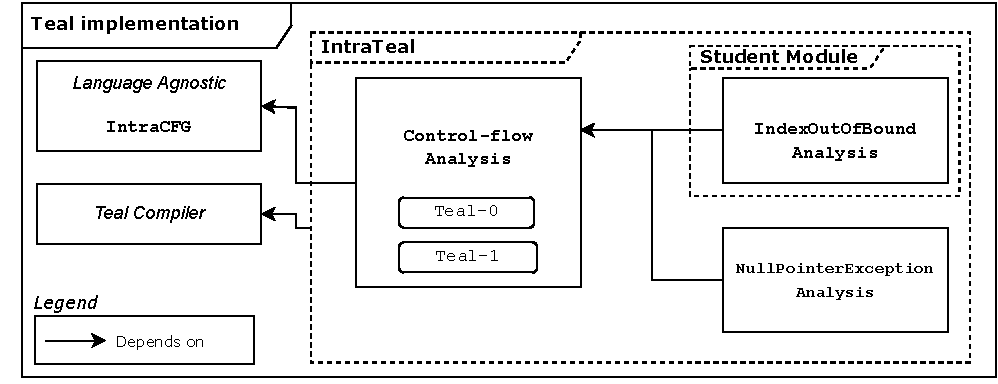
\includegraphics[scale=0.65]{kappa/img/architectureteal.pdf}
    \caption{\label{fig:IntraTeal} Overall architecture of \textsc{IntraCFG} instansiated for the Teal language.}
\end{figure}
As a further demonstration of the applicability of \textsc{IntraCFG},
we developed \textsc{IntraTeal}, an implementation of the framework for the Teal programming language.
The teal programming language is used for teaching purposes 
and provides a simple and easy-to-learn syntax for students to understand the 
concepts of static program analysis.
We made available to students, as part of the course, the complete source code of \textsc{IntraTeal}, 
with instructions and guidelines on how to use the API to implement their own analyses.
We also made available a reference implmentation of the 
\texttt{NullPointerException} analysis. We then asked students, as a way of 
extending their understanding and skills, to implement an \texttt{IndexOutOfBound} 
analysis on the interval abstract domain. This exercise provided the 
students with an opportunity to apply the concepts they had learned in a practical 
setting and gain a deeper understanding of dataflow analysis.

One of the key features of the \textsc{IntraTeal} implementation is that it 
constructs control-sensitive CFGs. Control-sensitive CFGs
are a more precise representation of the control flow of a program, as they take 
into account the specific control flow behavior of a program. This is achieved by
synthesizing  two new AST nodes, i.e., \texttt{ControlTrue} and \texttt{ControlFalse} for each
comparison operator, e.g.,  ``$\le$'', ``$==$'', ``$!=$'', inside a conditional statement.
These HOAs are used to represent the control flow of the program and the information that ca be inferred from 
it. \\
%
\begin{minipage}{0.45\textwidth}
    \begin{lstlisting}[language=JastAdd,caption={Control-sensitivity to improve null pointer analysis.}, label={lst:control-null}]
if(x!=null){
  //x is not null here
}
    \end{lstlisting}
    \end{minipage}\hfill%
    \begin{minipage}{0.45\textwidth}
    \begin{lstlisting}[language=JastAdd,caption={Control-sensitivity to improve interval analysis.}, label={lst:control-interval}]
if(x > 4 and x <= 6){
    //x is [5,6] here
}
    \end{lstlisting}
\end{minipage}\\
The example in Listing~\ref{lst:control-null} shows how the \texttt{ControlTrue} and \texttt{ControlFalse}
HOAs are used to keep track of the information that the object \texttt{x} is not null 
in the \emph{then} branch and null in the \emph{else} branch.
This information is used to improve the precision of the analysis and provide 
more accurate results without affecting the performance of the analysis.

We also asked students to use the \texttt{ControlTrue} and \texttt{ControlFalse} 
HOAs to improve the precision of the interval analysis. The example in
Listing~\ref{lst:control-interval} shows how the \texttt{ControlTrue} and \texttt{ControlFalse}
HOAs are used to keep track of the information that the object \texttt{x} is in the interval $[5,6]$.
\begin{figure}
	\centering
	\begin{tikzpicture}
		\node (a) at (0,0) {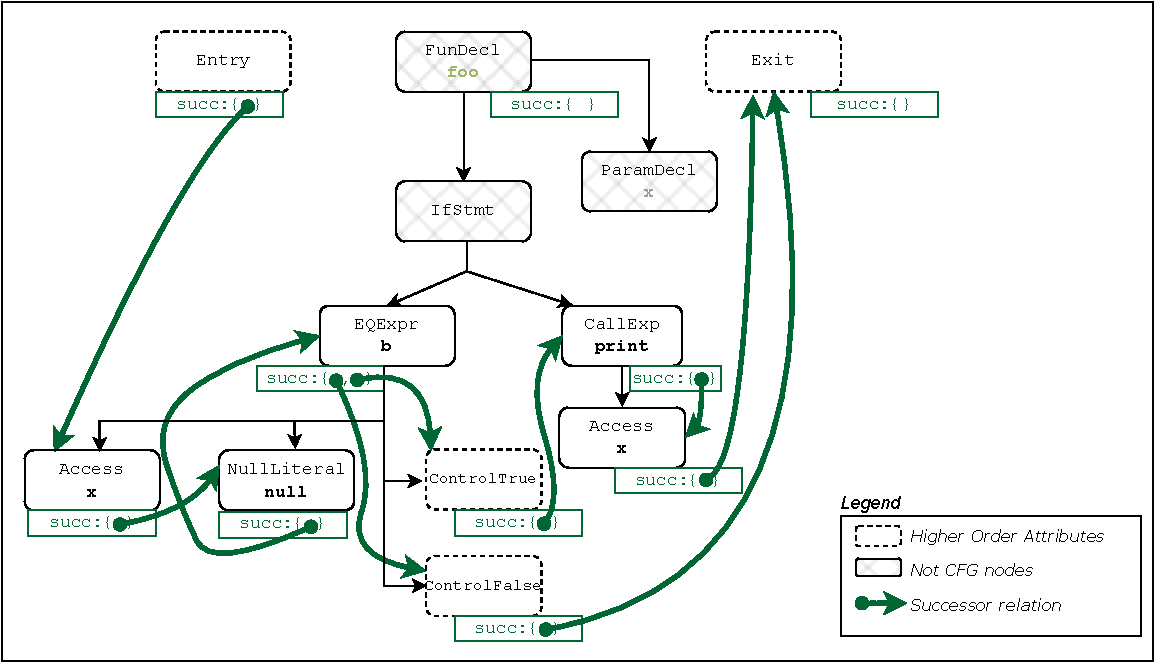
\includegraphics[scale=0.55]{kappa/img/TEALExample.pdf}};
		\node[scale=0.7] (b) at (3.5,0) {
			\begin{lstlisting}[language=JastAdd]
fun foo(x) = {
  if(x==null){
    print(x);
  }
}
			\end{lstlisting}
		};
	\end{tikzpicture}
	\caption{\label{fig:ExampleTEAL} Example of control-sensitivity in \textsc{IntraTeal}.}
\end{figure}
\begin{lstlisting}[language=JastAdd,label={lst:ControlTrueEq}, caption={Transfer function for \texttt{ControlTrue} HOA.}]
eq ControlTrue.nullnessTransfer(NullDomain lattice) {
  NullDomain result = new NullDomain(lattice);
  NullDomain assignment = getCond().getImplicitAssignment();
  return result.join(assignment);
}
\end{lstlisting}
The example presented in Figure~\ref{fig:ExampleTEAL} along with the code snippet
provided in Listing~\ref{lst:ControlTrueEq} illustrates how the precision of the
analysis is enhanced by considering implicit assignments in the control flow of 
the program. Specifically, the transfer function for the \texttt{ControlTrue} HOA
takes into account that the object \texttt{x} is null when it is printed within 
the \emph{then} branch of the \texttt{if} statement.


The task assigned to the students, which was an extension of the \texttt{NullPointerException}
analysis, was to implement an \texttt{IndexOutOfBound} analysis on the interval domain. 
The interval domain, being an infinite domain, poses a significant challenge for
dataflow analysis due to the inherent nature of infinite domains. In particular,
the iterative nature of dataflow analysis algorithms, which rely on the computation
of a sequence of approximations, may not terminate when applied to an infinite domain.
This can result in an excessive consumption of computational resources and ultimately
lead to a failure of the analysis. Additionally, the use of infinite domains can also
lead to the presence of non-converging sequences, resulting in an analysis that does
not converge to a stable solution. The example in Figure~\ref{fig:nonConverging}
illustrates a non-converging program.
\begin{figure}
	\centering
	\begin{tikzpicture}
		\node (a) at (3.5,0) {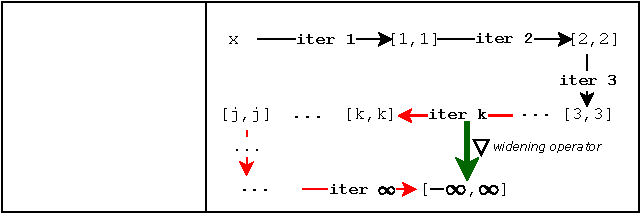
\includegraphics[scale=1]{kappa/img/non-convergin.pdf}};
		\node[scale=1] (b) at (-2,0) {
			\begin{lstlisting}[language=JastAdd]
fun foo(x) = {
  x := 0;
  while (true) {
    x = x + 1;
  }
}
			\end{lstlisting}
		};
	\end{tikzpicture}
	\caption{\label{fig:nonConverging} Trivial example of non-converging program.}
\end{figure}

To ensure the termination of the analysis, the students were required to 
define their own widening operator.
However, \textsc{JastAdd} circular attributes, which are used to implement dataflow 
analysis, do not natively support widening operators, as they are designed 
to work only on finite lattices. To overcome this limitation, an ad-hoc solution 
solution was implemented to trigger the widening operator after a certain 
number of steps.

This experience highlights the need for native support for widening and narrowing 
operators in \textsc{JastAdd}, to allow static analysis developers to effectively deal with 
infinite lattices. In the future, we plan to investigate the implementation of this 
feature in \textsc{JastAdd} to facilitate developers of static analysis tools.


\subsection{IDE Integration}
\subsubsection{LSP support via MagpieBridge: showing results and fixes}

\subsubsection{Visualisation and debugging via Codeprober}



\section{JFeature: A Java Feature Extractor}






\label{sec:contribution}
% In this Thesis, we present two major contributions to the field of programming 
% language analysis and software engineering. 
% The first significant contribution of this thesis is the formalisation of \textsc{IntraCFG},
% a language-agnostic RAG-based framework for constructing control-flow graphs (CFGs) 
% on top of the abstract syntax tree (AST). \textsc{IntraCFG}, is a highly flexible
% framework that enables the construction of light-weight and precise the control-flow graphs
% of a program. To exemplify the applicability of \textsc{IntraCFG}, we instantiate it for the TEAL language.

% The second contribution is a Java feature extractor called \textsc{JFeature}.
% This tool is designed to assist researchers in selecting the appropriate corpora
% for their experiments by extracting relevant features from Java programs. 
% \textsc{JFeature} is able to extract a wide range of features, 
% including syntactic, e.g., use of keywords, and semantic features, e.g.,
% the number of method calls.


% \subsection{\textsc{IntraCFG}: A Precise Framework for Source-level Control-flow Analysis}

% \subsubsection*{Design and Implementation}
% \textsc{IntraCFG} is written within the \textsc{JastAdd} ecosystem.

% The framework provides three interfaces, namely \code{CFGRoot}, \code{CFGNode}, and \code{CFGSupport},
% to be implemented by AST nodes. Each interface provides a set of attribute that are used to construct
% the CFGs.

% The \code{CFGRoot} interface is the starting point of the CFG construction process.
% It is implemented by AST nodes that identify the subtree containing the entire method 
% or function. This interface is responsible for defining the entry and exit nodes of the CFG and 
% forwards a reference of the entry node to every \code{CFGNode}.


% The \code{CFGSupport} interface is implemented by nodes that are not part of the CFG,
% but define its shape. These nodes are used to provide additional information 
% about the structure of the CFG, such as the presence of loops or branches. 
% They are designed to be used as auxiliary nodes to support the CFG construction 
% process, and they do not participate directly in the control-flow.